\documentclass[12pt]{article}

\usepackage{sbc-template}
\usepackage{graphicx,url}
\usepackage[utf8]{inputenc}
\usepackage[brazil]{babel}
\usepackage{lipsum}
\usepackage{hyperref}
\usepackage{colortbl}
\usepackage{pgf, tikz}
\usepackage{multirow}
\usepackage[toc,page]{appendix}
\usepackage{afterpage}

\addtolength{\intextsep}{-1pt}

\sloppy

\title{SaaS para gestão de condomínio - Condomínio Madre Paulina}

\author{William S. Nepomuceno\inst{1}}

\address {
    Instituto de Tecnologia -- Universidade de Passo Fundo
    (UPF) \\
    Passo Fundo -- RS -- Brazil
    \email{178344@upf.br}
}

\begin{document}

\maketitle

\begin{abstract}
The present work presents the proposal of a SaaS for the management of condominiums, based on the needs of the Madre Paulina condominium and also the development of improvements for the WEB platform that the condominium already has. Initially, the requirements and use cases raised with end users will be described. Based on the requirements raised, the application was modeled based on the application of the concepts of Clean Architecture and its layers and the SOLID Principles, all of this being developed test-oriented. Finally, there will be a brief presentation of the WEB platform and the application, showing its main features.
\end{abstract}

\begin{resumo} 
O presente trabalho apresenta a proposta de um SaaS para a gestão de condomínios, baseado nas necessidades do condomínio Madre Paulina e também o desenvolvimento de melhorias para a plataforma WEB que o condomínio já possuí. Inicialmente será descrito os requisitos e casos de usos levantados com os usuários finais. Com base nos requisitos levantados foi realizado a modelagem da aplicação a partir da aplicação dos conceitos de Clean Architeture e suas camadas e dos Princípios SOLID, tudo isso sendo desenvolvido orientado a testes. Por fim terá uma breve apresentação da plataforma WEB e do aplicativo, mostrando suas principais funcionalidades.

\end{resumo}

\section{Introdução}
Este projeto tem como objetivo o desenvolvimento de um SaaS (Software as Service) para gestão de condomínios, baseado nas necessidades do condomínio Madre Paulina.

\subsection{Contextualização}
Atualmente o condomínio Madre Paulina conta com com quinze condôminos, sendo duas salas comerciais, devido ao grande número de condôminios para facilitar a gestão,
o condominío já conta com uma plataforma WEB para o gerenciamento de suas atividades, desenvolvida por mim durante a disciplina de Laboratório de Engenharia de Software em 2022/1.

O backend da plataforma WEB foi desenvolvido utilizando o framework Laravel e o frontend utilizando o framework Angular, que se comunicam através de uma API REST.
Tanto o backend quanto o frontend estão hospedados no Heroku, que é uma plataforma de hospedagem de serviços web. Para o banco de dados foi utilizado o SGBD MySQL, atualmente hospedado nos serviços RDS da Amazon Web Services.

O aplicativo será desenvolvido utilizando a linguagem de programação Dart e o framework Flutter, que permite o desenvolvimento de aplicações móveis nativas para Android e iOS, que também irá se comunicar com o backend através de uma API REST.

\subsection{Motivação}
A partir do cenário atual do condomínio Madre Paulina, aliado com o crescimento da demanda contábil sobre a administração de condomínios onde é cada vez mais necessário obter informações precisas para a tomada de decisão, para evitar um défict nas contas do condomínio e levando em consideração que no condomínio ainda são realizados de forma manual em cadernos, causando transtornos na prestação de contas, pela perda de informações, urge a necessidade de uma ferramenta que possibilite e facilite a contabilidade do condomínio Madre Paulina de forma mais precisa.

\subsection{Limitações}
A publição do aplicativo está limitado somente à plataforma Android.

\section{Modelagem da aplicação}
Na base da modelagem dos projetos estão os seus requisitos, é fundamental que ao se desenvolver um sistema saibamos quais as necessidades das partes interessadas: usuários, clientes, fornecedores, desenvolvedores, empresas e o que o sistema deverá fazer para satisfazer essas necessidades.

Também é importante ponderar que os requisitos da aplicação disponibilzaram a base para o planejamento do desenvolvimento do sistema, bem como critérios para testes.

\subsection{Requisitos do sistema}
Requisitos definem o que um sistema deve fazer e sob quais restrições. Requisitos relacionados com a primeira parte dessa definição — o que um sistema deve fazer, ou seja, suas funcionalidades, ou até mesmo o que um sistema não deve fazer — são chamados de Requisitos Funcionais. Já os requisitos relacionados com a segunda parte — sob que restrições — são chamados de Requisitos Não-Funcionais \cite[Capítulo 3.1]{engsoftware}.

Após o levamento dos requisitos com o usuário final da aplicação, foram identificados os seguintes Requisitos Funcionais \ref{Req-func} e Requisitos Não-Funcionais \ref{Req-nfunc}.

\subsubsection{Requisitos Funcionais}
\label{Req-func}
Nesta seção serão descritos os dois principais requisitos funcionais solicitados pelo usuário final.

\begin{center}
\begin{tabular}{| p{0.18\textwidth} | p{0.75\textwidth} |}
  \hline
  RF-001 & Adicionar usuário \\
  \hline
  RF-002 & Editar usuário \\
  \hline
  RF-003 & Adicionar período \\
  \hline
  RF-004 & Adicionar receita/despesa em um período \\
  \hline
  RF-005 & Remover receita/despesa de um período \\
  \hline  
\end{tabular}
\end{center}

Inicialmente estava previsto também o desenvolvimento de outras duas funcionalidades, sendo a Reversa do Salão de Festas e Atas de Assembleia, porém os usuários finais não chegaram em um conceso quanta a regras e definições. 

Outras funcionalidades, como a Integração com o Internet Baking para a geração dos boletos do condominío, não foram desenvolvidas por falta de tempo.

\subsubsection{Requisitos Não-Funcionais}
\label{Req-nfunc}
Nesta seção serão descritos os dois principais requisitos não-funcionais.

\begin{center}
\begin{tabular}{| p{0.18\textwidth} | p{0.75\textwidth} |}
  \hline
  \multicolumn{2}{|c|}{\cellcolor{gray!30}Segurança} \\
  \hline
  RNFSEG-001 & Apenas usuários cadastrados deverão ter acesso ao sistema, 
  por meio de login. \\
  \hline
  RNFSEG-002 & As requisições deverão ser autenticadas por meio de Json Web Token. \\
  \hline
  RNFSEG-003 & As senhas dos usuários deverão estar criptografadas. \\
  \hline
  \multicolumn{2}{|c|}{\cellcolor{gray!30}Interface} \\
  \hline
  RFNINT-001 & O aplicativo deve ter uma interface visual de fácil compreensão, para que não haja treinamento prévio dos usuários. \\
  \hline
\end{tabular}
\end{center}

\subsection{Casos de usos}
Casos de uso (use cases) são documentos textuais de especificação de requisitos. Um caso de uso enumera os passos que um ator (usuário) realiza em um sistema com um determinado objetivo. Um caso de uso inclui duas listas de passos, sendo a primeira o fluxo normal, que são os passos necessários para concluir uma operação com sucesso. A segunda representa extensões desse fluxo normal, geralmente casos de exeções \cite[Capítulo 3.1]{engsoftware}.

Os casos de uso da aplicação, bem como o seu diagrama estão descritos no Apêndice \ref{appendice_use_case}.

\section{Desenvolvimento do Aplicação}
Para garantir uma boa qualidade de código, o projeto foi desenvolvido utilizando os princípios do Test Driven Development (TDD) explanados na seção \ref{TDD}, que consiste em escrever os testes antes do código. Outro principio utilizado para desenvolvimento da aplicação foi o SOLID, que consiste em 5 princípios de orientação a objetos que devem ser seguidos para garantir uma boa qualidade de código. As seções abaixo apresentam os detalhes destes principios aplicados ao projeto.

\subsection{Test Driven Development}
\label{TDD}
Test Driven Development (TDD), ou Desenvolvimento Orienteado a Testes, é uma prática de desenvolvimento de software sugerida por diversas metodologias ágeis, como o XP. A ideia sugere  aos desenvolvedores que os escrevam testes automatizados de maneira contínua, ao longo do desenvolvimento do software.

Porém a ideia do TDD é que os desenvolvedores escrevam os testes antes da implementação do código, garantindo assim que o código seja testado. Dessa forma a suíte de testes é maior, abrangindo mais casos de testes \cite[Capítulo 8.1]{engsoftware}.

Aplicando a prática do TDD para desenvolver este projeto foi possível obter uma cobertura de testes de cerca de 85\%.

\section{Arquitetura}
Para o desenvolvimento da aplicação foi adotada arquitetura em camadas é um dos padrões arquiteturais mais usados, desde que os primeiros sistemas de software de maior porte foram construídos nas décadas de 60 e 70. Em sistemas que seguem esse padrão, as classes são organizadas em módulos de maior tamanho, chamados de camadas. As camadas são dispostas de forma hierárquica, como em um bolo. Assim, uma camada somente pode usar serviços — isto é, chamar métodos, instanciar objetos, estender classes, declarar parâmetros, lançar exceções, etc. — da camada imediatamente inferior \cite[Capítulo 7.2]{engsoftware}. 

Conjutantamente com a arquitetura em camadas, foi aplicado os conceitos de Clean Architecture definidos por Robert C. Martin em seu livro Clean Architecture: A Craftsman's Guide to Software Structure and Design, publicado em 2017 \cite{cleanArchitecture}.

\subsection{Clean Architecture}
Clean Architecture ou também chamada de Arquitetura Limpa é um padrão de projeto de software para arquitetura de software que segue os conceitos de código limpo e implementa princípios SOLID \ref{SOLID}.

Os padrões de projeto podem ser definidos como boas práticas que ajudam a manter a lógica de negócios unida para minimizar as dependências dentro do sistema. Seguindo a arquitetura limpa permite aos arquitetos de software desacoplar componentes para que fiquem isolados o suficiente para serem duráveis e facilmente alterados sem refazer o sistema.

Dessa forma, seguindos estas boas práticas foi elaborada a proposta de arquitetura para o requisito RF001 - Adicionar um novo usuário \ref{Req-func} está representada através de um diagrama na Figura \ref{fig:DiagramaArquitetura}.

\begin{figure}[!ht]
  \centering
  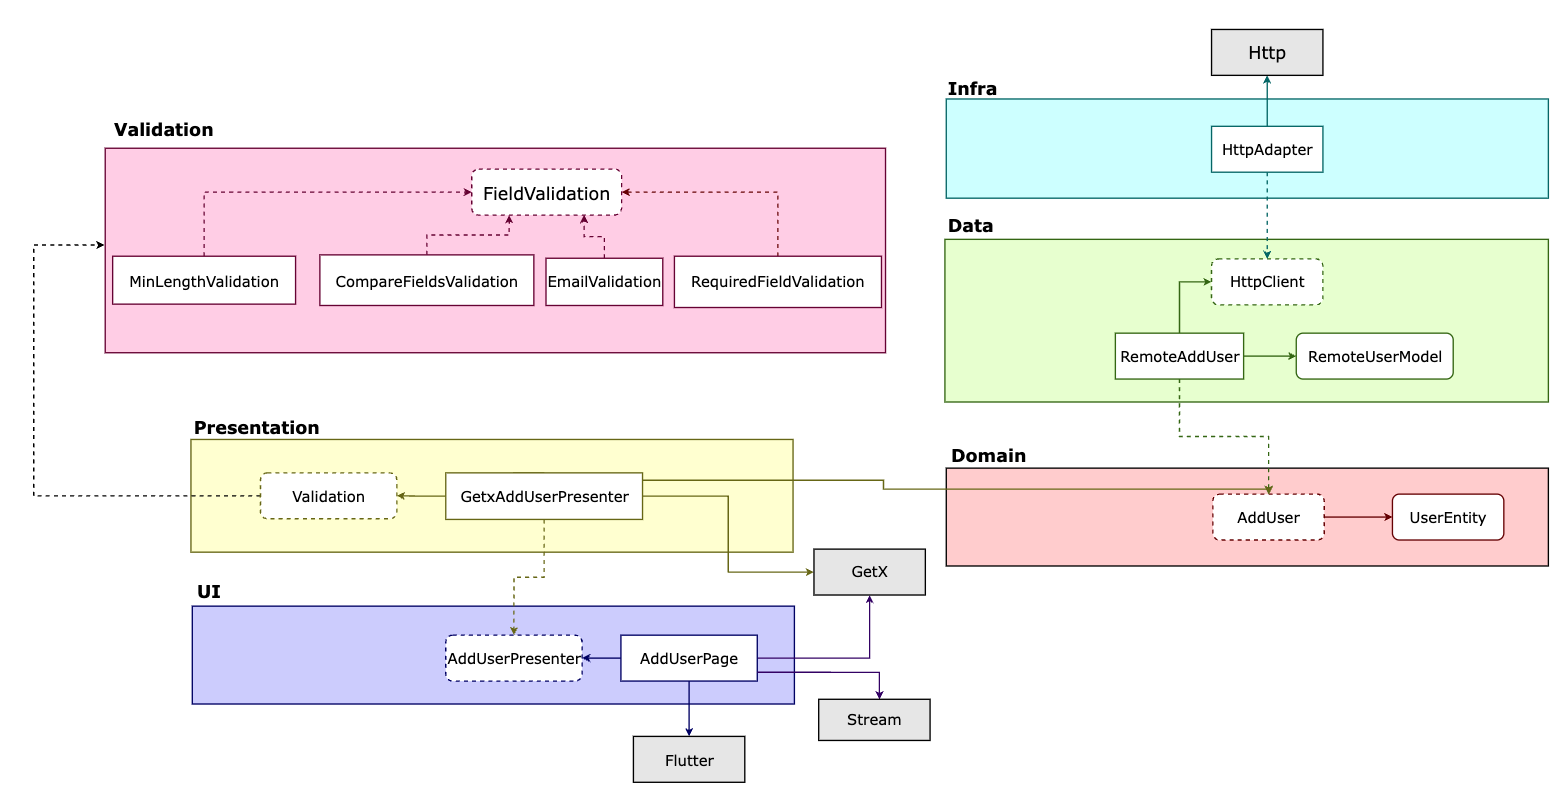
\includegraphics[width=\textwidth,height=\textheight,keepaspectratio]{projeto/images/DiagramaArquitetura.png}
  \caption{Proposta de Arquitetura para a aplicação.}
  \label{fig:DiagramaArquitetura}
\end{figure}

\subsection{Camadas}
As camadas (layers) são o núcleo principal para arquitetura limpa. 
Para o desenvolvimento do aplicativo, foi utilizado sete camadas: Domain, Data, Infra, Main, Presentation, UI, Validation.

\subsubsection{Domain Layer}
\label{domainLayer}
A camada de domínio ou domain layer é uma abastração responsável por encapsular as regra de negócios do sistema e forncer casos de usos. Para manter essas classes simples, cada caso de uso deve ter responsabilidade apenas sobre uma única funcionalidade \ref{SRP} e não deve conter dados mutáveis. Em vez disso, os dados devem ser manipulados na camadas de dados \ref{dataLayer}.

Ao utilizar camada de domínio é possível obter alguns benefícios, como:
\begin{itemize}
    \item Pemitir a divisão de responsanbilidade.
    \item Reduzir a duplicação de código.
    \item Melhorar a testabilidade do aplicativo.
\end{itemize}

\subsubsection{Data Layer}
\label{dataLayer}
Camada de dados ou data layer é responsável por acessar os dados de alguma fonte, seja ela um banco de dados, um arquivo, uma API, etc.

Está camada implementa as regras de negócios definidas pela camada de domínio, ou seja, ela não deve conter nenhuma regra de negócio, apenas implementar as regras definidas pela camada de domínio.

\subsubsection{Infra Layer}
\label{infraLayer}
Camada de infraestrutura é responsável por se comunicar com serviços externos, como por exemplo, um banco de dados, uma API, ou seja, qualquer serviço externo que a aplicação precise se comunicar, por meio de interfaces. Neste projeto a camada de infraestrtura é responsável por se comunicar com a API e também com a memória cache dos dispositivos.

\subsubsection{Main Layer}
\label{mainLayer}
Nesta camada é realizada a composição das camadas, por meio de injeção de dependência, ou seja, a camada principal é responsável por injetar as dependências de cada camada, e também é responsável por inicializar a aplicação. 

Em casos de uma API, esta camada é responsável por inicializar o servidor web e expor as rotas da aplicação.

\subsubsection{Presentaion Layer}
\label{presentantionLayer}
Camada de apresentação ou presentation layer é responsável por expor a aplicação para o usuário, seja ela uma API, um site, um aplicativo, etc. Neste projeto, também é a camada responsável por executar as ações do usuário, como por exemplo, receber os dados de um formulário. 

Em casos de uma API, esta camada é responsável por receber os dados da requisição, realizar o processamento dos dados, sejam eles salvar no banco de dados, ler do banco de dados, enviar para uma API externa, etc. E também é responsável por retornar os dados para o usuário, seja eles um JSON, um XML, um HTML, etc.

\subsubsection{UI Layer}
\label{uiLayer}
Camada de interface ou UI layer é a camada onde o usuário interage com a aplicação. Neste projeto, a camada de interface é responsável por exibir os dados para o usuário, e também é responsável por receber as ações do usuário, como por exemplo um formulário, um botão, etc.

A inteface do aplicativo foi desenvolvida utilizando a biblioteca Flutter Material, que são widgets que implementam o Material Design. Atualmente, o aplicativo conta com um menu lateral, que permite ao usuário acessar as funcionalidades do aplicativo, como:

\begin{itemize}
    \item Início: Página inicial do aplicativo.
    \item Usuários: Página que exibe as informações do usuário, permitindo adicionar novos usuários e editar os já existentes.
    \item Fluxo de Caixa: Página que exibe as informações do fluxo de caixa, permitindo lançar novas receitas e despesas para um período e exibe os lançamentos de forma sumarizada.
\end{itemize}

Mais detalhes sobre a interface e funcionalidades do aplicativo estão descritas na seção \ref{mobile_application}.

\subsubsection{Validation Layer}
\label{validationLayer}
É a camada responsável por realizar a validação de dados informados pelo usuário na camada UI. Para o projeto foi implementada a validação de tamanho mínimo de um campo, e-mail, CPF, senha e confirmação de senha.

\subsection{Princípios SOLID}
\label{SOLID}
Os princípios SOLID são cinco princípios de programação orientada a objetos e design de código que ajudam a tornar os programas mais fáceis de entender, manter e estender. Os princípios SOLID foram definidos por Robert C. Martin em seu livro Clean Architecture \cite{cleanArchitecture}, os 5 princípios que compõe o SOLID são:
 
\subsubsection{S - Single Responsibility Principle (Princípio da Responsabilidade Única)}
\label{SRP}
\lipsum[1]

\subsubsection{O - Open/Closed Principle (Princípio Aberto/Fechado)}
\label{OCP}
\lipsum[1]

\subsubsection{L - Liskov Substitution Principle (Princípio da Substituição de Liskov)}
\label{LSP}
\lipsum[1]

\subsubsection{I - Interface Segregation Principle (Princípio da Segregação da Interface)}
\label{ISP}
O Interface Segregation Principle (ISP) nó diz que uma classe não deve ser forçada a implementar uma interface que ela não irá utilizar. O ISP é um princípio que nos ajuda a manter nossas classes mais coesas e focadas em uma única responsabilidade.

Um exemplo de ISP  é o uso de interfaces ou classes abstratas. Uma interface é um contrato que define um conjunto de métodos que uma classe deve implementar. Uma classe pode implementar várias interfaces, mas uma interface não pode ser implementada por várias classes.

Neste projeto uma aplicação deste princípio é o módulo SecureStorageAdapter \autoref{fig:SecureStorageAdapter}, que é responsável pela comunicação com a memória cache dos dispositivos. Como é possível salvar, ler e deletar os dados da memória cache, foi feita a segração das ações três interfaces \autoref{fig:SecureStorageInterfaces}, dessa forma se o módulo SecureStorageAdapter não necessitasse mais da ação deletar, basta remover a implementação da interface. 

\begin{figure}[!ht]
  \centering
  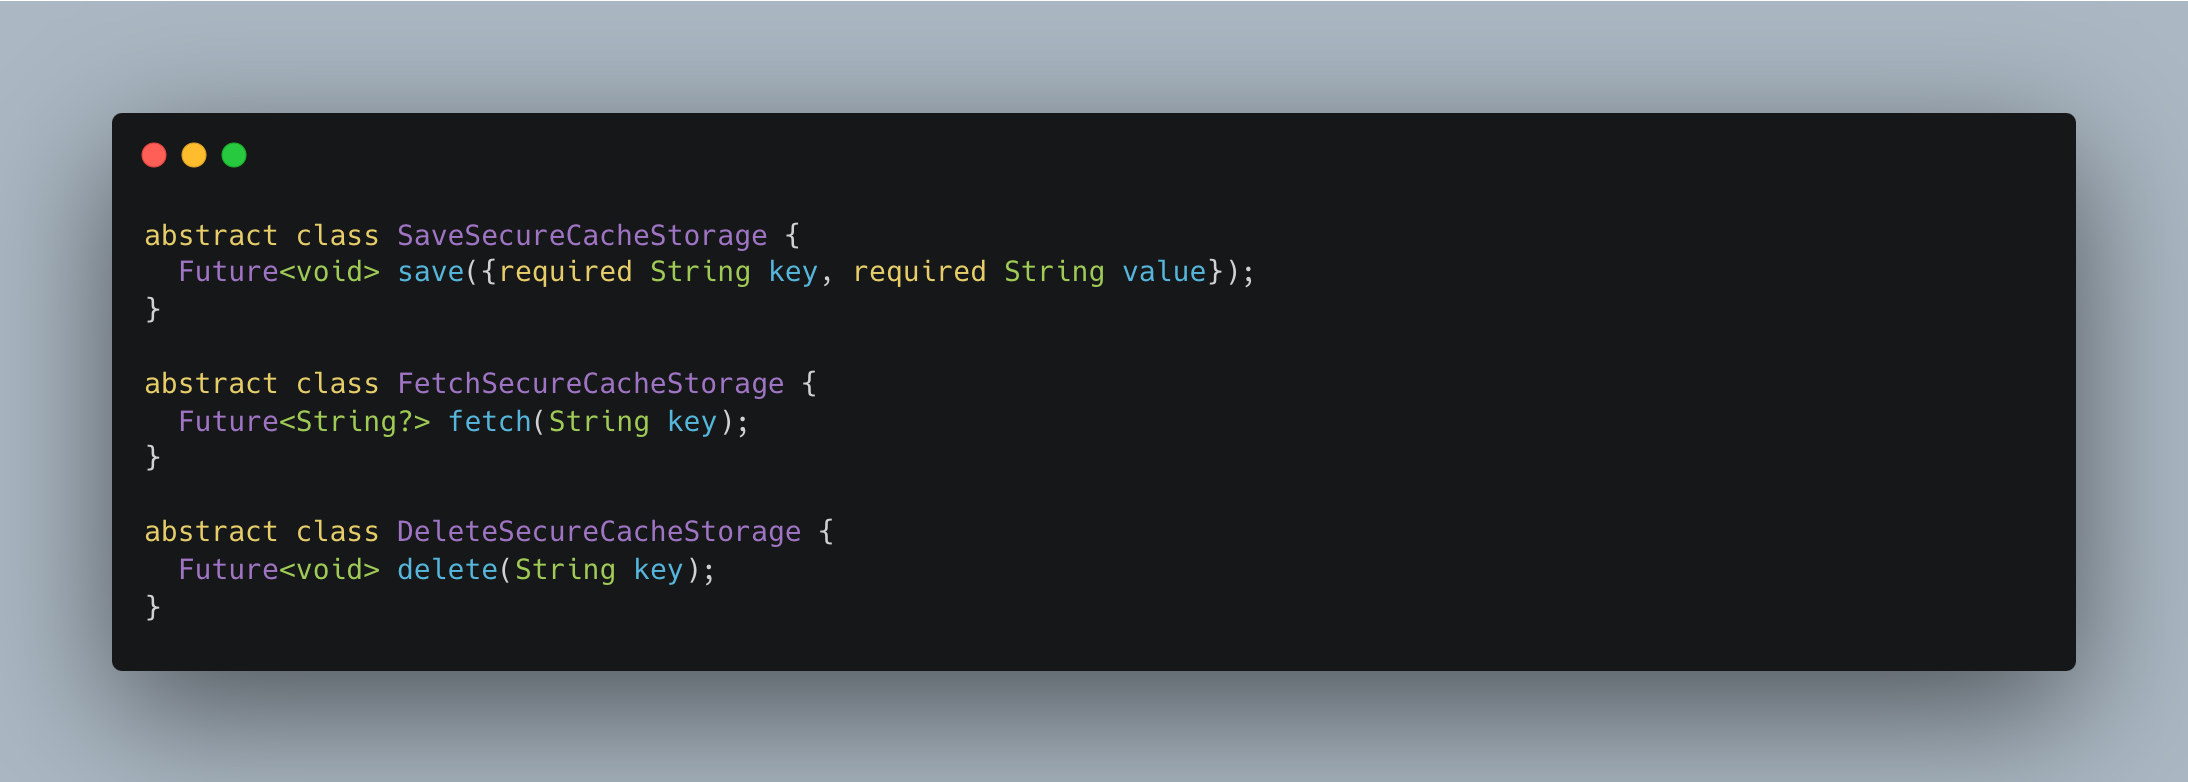
\includegraphics[width=\linewidth]{projeto/images/secure_storage.png}
  \caption{Interfaces SecureStorage}
  \label{fig:SecureStorageInterfaces}
\end{figure}

\begin{figure}[!ht]
  \centering
  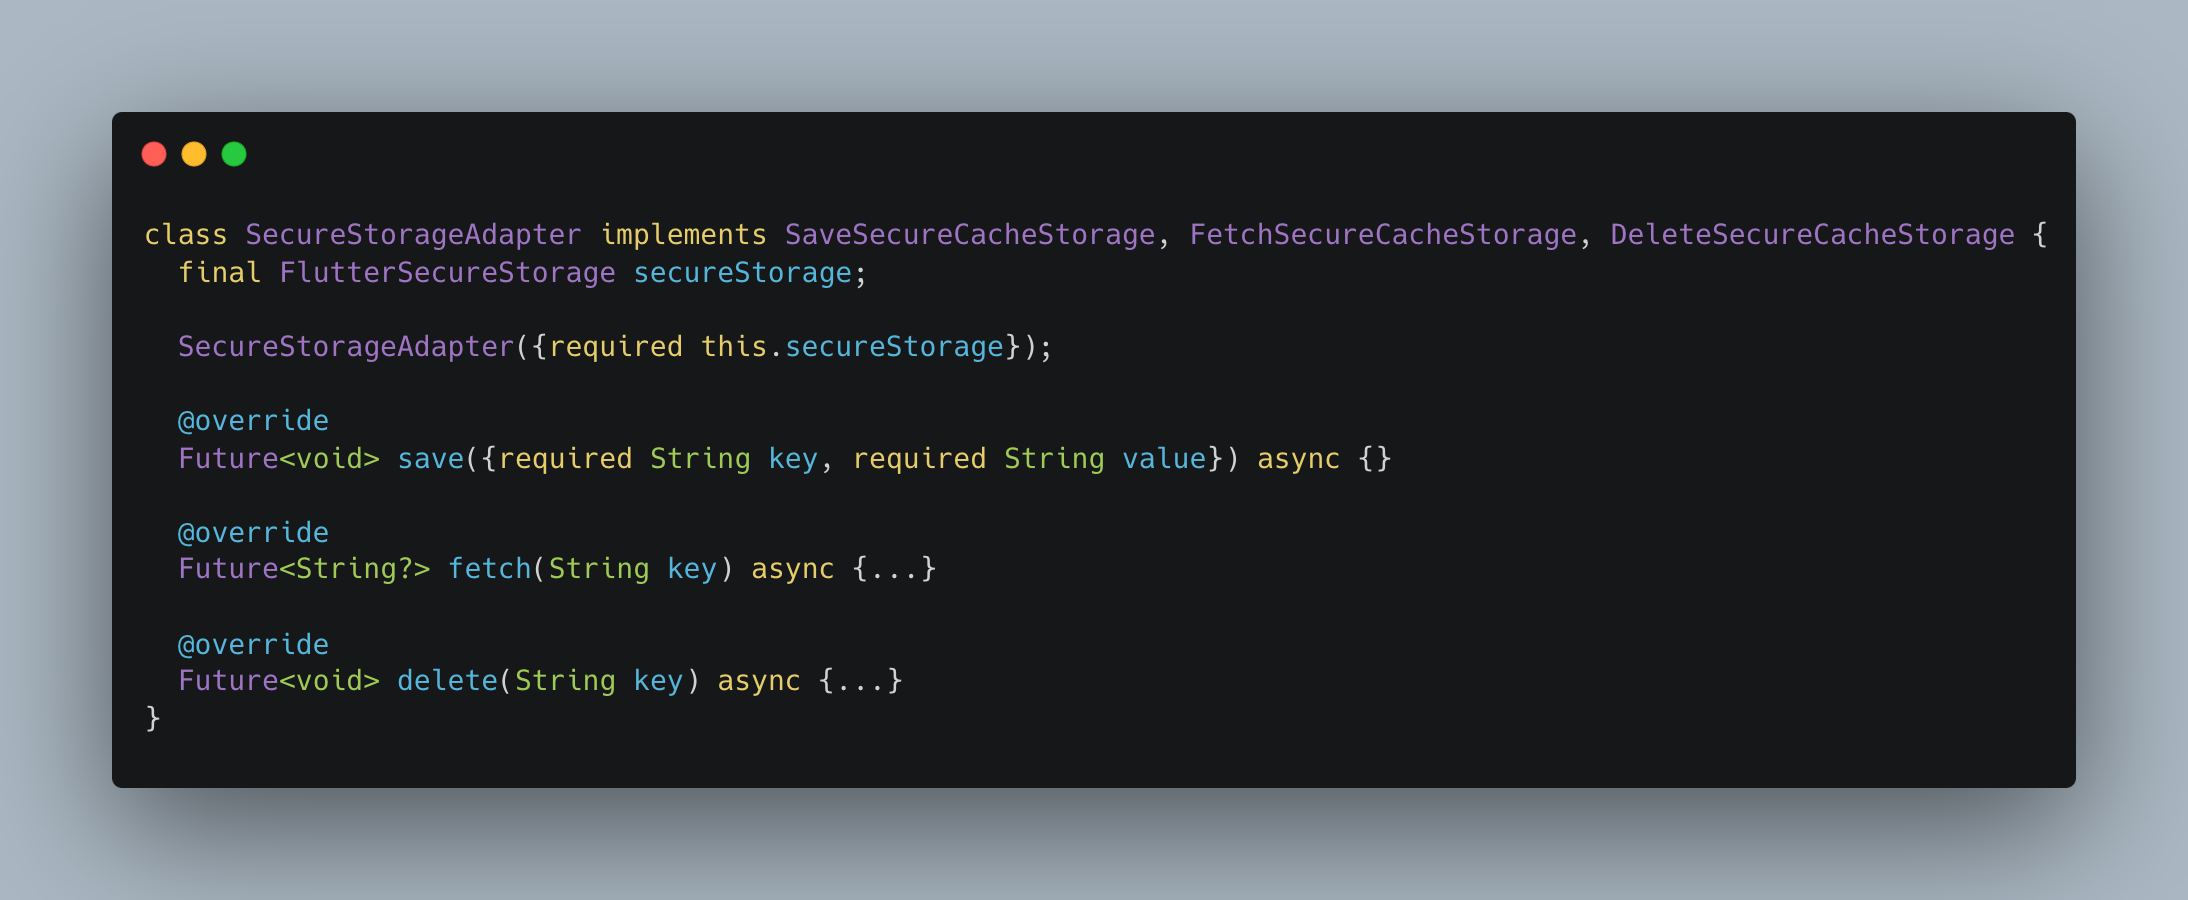
\includegraphics[width=1\linewidth]{projeto/images/secure_storage_adapter.png}
  \caption{Implementação SecureStorageAdapter}
  \label{fig:SecureStorageAdapter}
\end{figure}

\subsubsection{D - Dependency Inversion Principle (Princípio da Inversão da Dependência)}
\label{DIP}
O Dependency Inversion Principle (DIP) nos diz que os módulos de alto nível não devem depender de módulos de baixo nível. Ambos devem depender de abstrações e as abstrações não devem depender de detalhes.

Um exemplo de DIP, assim como no ISP é o uso de interfaces, ou seja, uma classe pode depender de uma interface, mas não de uma implementação concreta. Isso permite que a classe seja usada com qualquer implementação da interface, não apenas com a implementação que foi projetada para ser usada com ela, permitindo que a classe seja testada de forma isolada.

Neste projeto uma aplicação deste princípio é o caso de uso AddAccount, onde é feita a injenção da classe abstrata HttpClient \autoref{fig:DIPHttpClient} e não da classe concetra HttpAdapter responsável por realizar as requisições Http \autoref{fig:httpClientInterface}.

\begin{figure}[!ht]
  \centering
  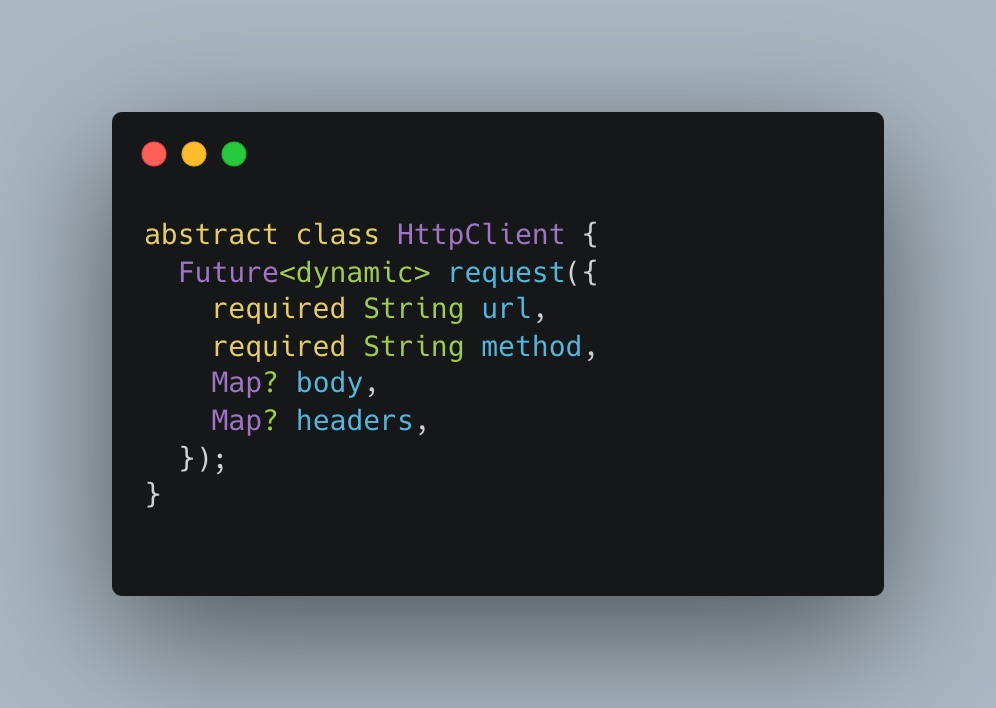
\includegraphics[width=0.7\columnwidth]{projeto/images/http-client.png}
  \caption{Interface para o módulo de requisições Http}
  \label{fig:httpClientInterface}
\end{figure}

\begin{figure}[!ht]
  \centering
  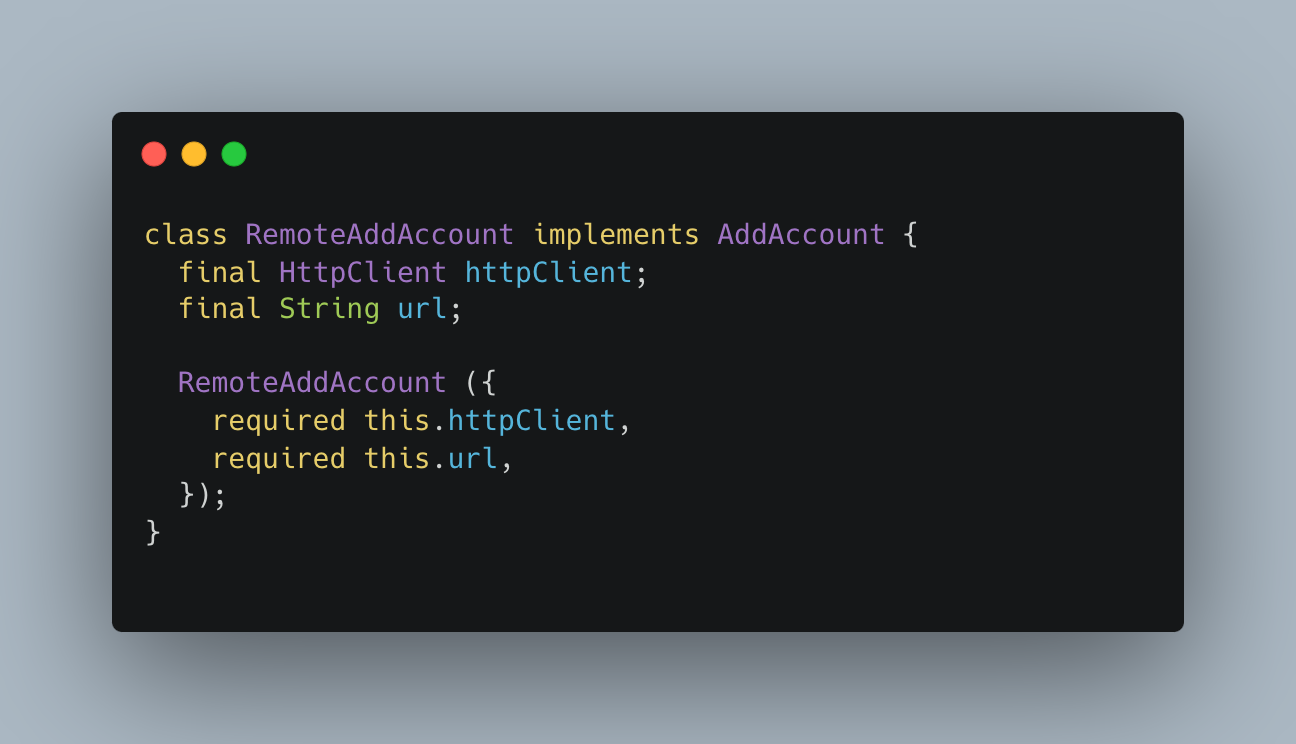
\includegraphics[width=0.7\columnwidth]{projeto/images/remote-add-addcount.png}
  \caption{Injenção da dependência HttpClient}
  \label{fig:DIPHttpClient}
\end{figure}

\section{Plataforma WEB}
A plataforma WEB permite ao síndico gerenciar o condomínio e seus respectivos condôminos, nele também é possível gerenciar os valores do condomínio, algumas taxas básicas, como uso do salão de festas, taxa de mudança e outros valores referentes ao m³ da água e valor para a geração do boleto, conforme a  \autoref{fig:UI_condominio}.

Outra funcionalidade presente na plataforma, é a tela para realizar o gerencimaneto da leitura d’água de um período, \autoref{fig:UI_Geracaoagua}, sendo possível gerenciar o consumo d’água para cada apartamento, por meio de um cálculo automático, que considera o consumo feito na úlitma leitura e acresce os valores das taxas básicas, e se houverem, também podem ser adicionado os valores referentes às taxas de uso de salão de festas e mudanças. Após a geração dos boletos no Internet Baking é possível anexá-los, para que os condôminos possam visualizar os boletos por meio de um relatório.

A plataforma também dispõe um relatório, onde os condôminos podem acessar e acompanhar o seu consumo mensal d'àgua por meio de um gráfico de barras, \autoref{fig:UI_graph_consumo}, e também visualizar os boletos do condomínio, \autoref{fig:UI_report_consumo}. Neste relatório caso o usuário possua o perfil Condômino, será exibido apenas os dados referentes ao seu apartamento, para usuários com o perfil de Síndico e Administrador, existe a possibilidade de aplicar um filtro por condômino.

Outro relatório administrativo que está presenta na plataforma é o de Relatório de Receitas e Despesas, \autoref{fig:UI_report_cashflow}. Neste relatório será possível visualizar as receitas/desepsas e o saldo mensal de um ano.

Na plataforma também está disponível as funcionalidades referentes a cadastro de usuário e seu respectivo perfil e permissões.

\section{Aplicativo Móvel}
\label{mobile_application}
O aplicativo móvel permite ao síndico realizar o controle do fluxo de caixa do condomínio, lançando receitas e despesas a partir de um cadastro de períodos (mês) \autoref{fig:UI_add_period}.

Após realizar o cadastro de um período é possível fazer o lançamento de receitas/despesas, \autoref{fig:UI_add_period_details}, por meio de um formuário onde é necessário informar uma Descrição, Valor, Ddata e Tipo (Entrada / Saída).

Através do aplicativo também é possível visualizar o balanço mensal, \autoref{fig:UI_Period_Details}.

\section{Conclusões}
O presente projeto teve como objetivo o desenvolvimento de uma plataforma para o condomónio Madre Paulina. Durante o desenvolvimento procurou-se respeitar os requisitos funcionais e não-funcionais levantados com os usuários. 

Dessa o projeto abre caminho para que o condominío Madre Paulina e futuramente outros condominíos possam utilizar uma plataforma de análise e planejamento para melhorar tomadas de decisões, reduzindo custos, por exemplo.

Por outro lado, com o desenvolvimento orientado a testes, aplicando os princípios de Clean Architeture e SOLID, acredite-se que será possível adicionar de forma tranquila, novas funcionalidade para o aplicativo. 

A aplicação destes conceitos e princípios também será de grande valia para a carreira profissional, tendo vista que o mercado da tecnologia da informação está cada vez mais exigente.

\section{Trabalhos Futuros}
Em função da indecisão de alguns requisitos e do curto prazo de tempo para a conclusão deste projeto, recomenda-se para trabalhos futuros o desenvolvimento da integração com o Internet Banking para a geração dos boletos, visto que atualmente a geração dos boletos  está sendo feita de forma manual, se tornando uma atividade morosa.

Outro ponto interessante para empreender um esforço, seria o de realizar um estudo sobre plataformas de hospedagem de serviços, considerando que a partir de novembro o Heroku não oferecerá mais serviços gratuitos.

Por fim, sugere-se a retomada com os usuários finais referentes as funcionalidades de Reversa do Salão de Festas e de Atas de Assembleia para definir as regras de negócio e posteriormente implementá-las.

\bibliographystyle{acm}
\bibliography{bibliography}

\newpage 

\begin{appendices}

\section{Casos de usos}
\label{appendice_use_case}
Nesta seção estão detalhados os principais casos de uso levantados para atender a solução proposta. A \autoref{fig:UC_Diagram} representa o diagrama de casos de uso, onde se pode ver de maneira resumida cada caso de uso e seus respectivos relacionamentos.

\begin{figure}[!ht]
  \centering
  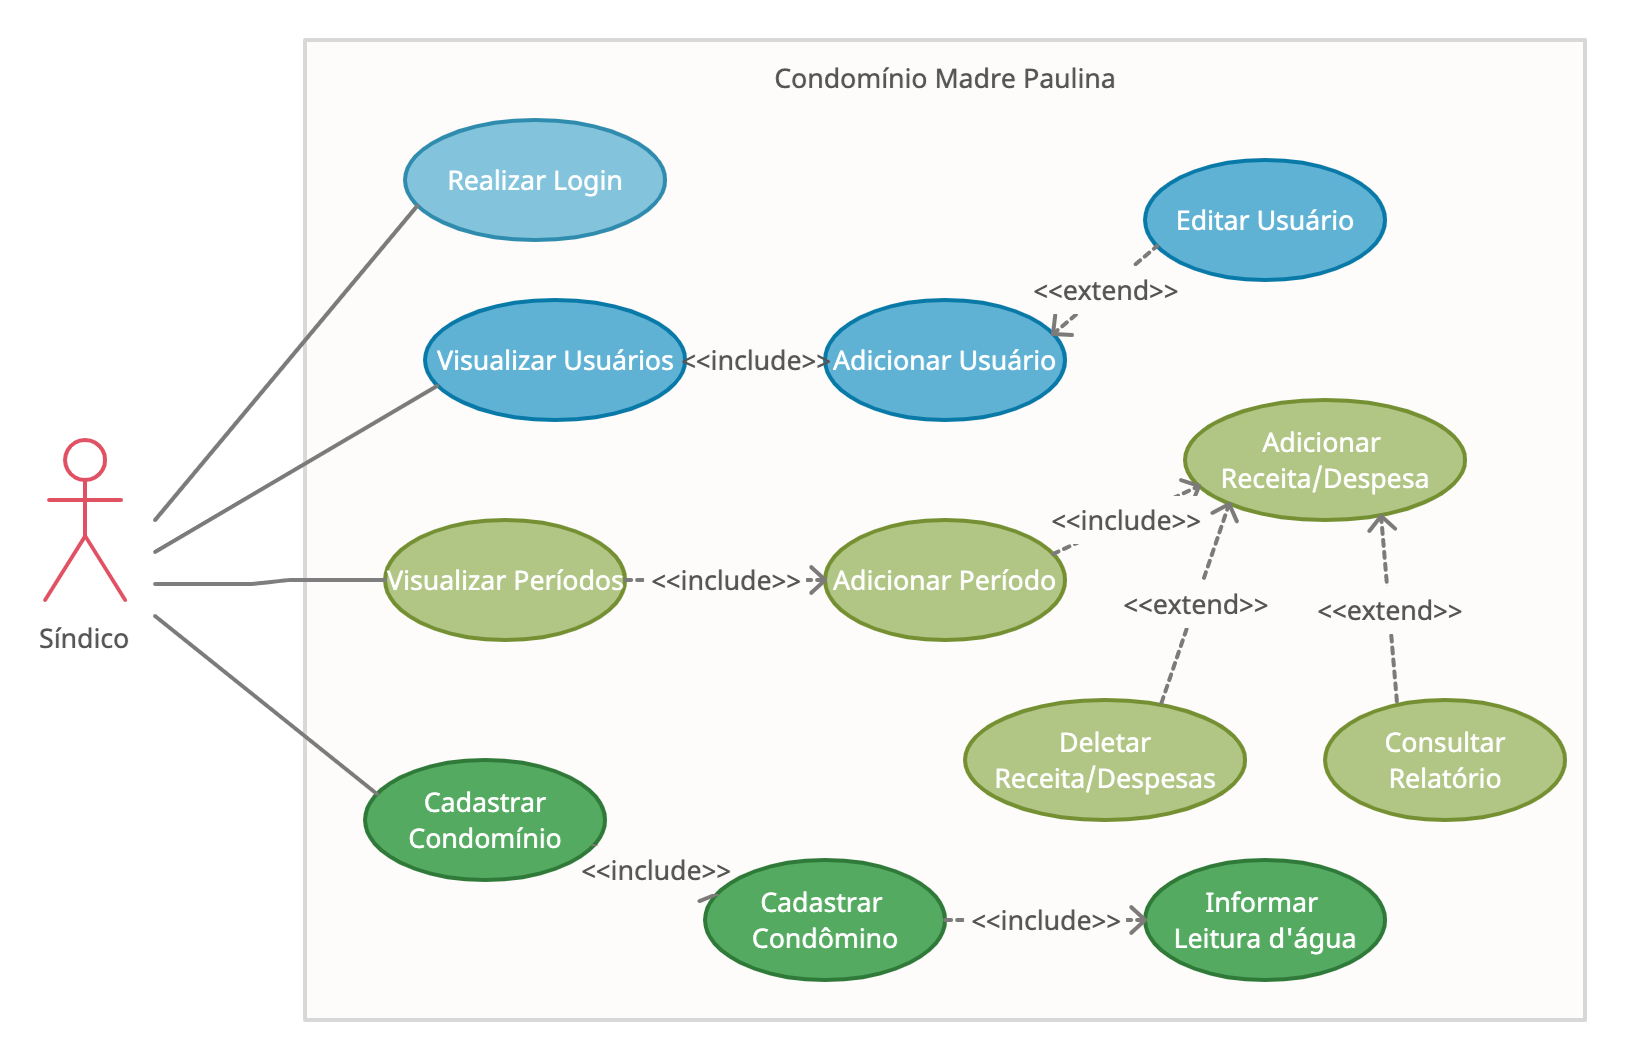
\includegraphics[width=1\columnwidth]{projeto/images/UC_Diagram.png}
  \caption{Diagrama Casos de Uso Aplicativo}
  \label{fig:UC_Diagram}
\end{figure}

\subsection{RF001 - Adicionar Período}
\label{sec:rf001}
O usuário na condição de síndico, deve ter a possibilidade de adicionar um novo período. O cadastro deste período deve ser por meio de um formulário, o usuário deve informar um Nome, Data Ínicio, Data fim e Status (Aberto / Fechado). Após a submissão os dados devem ser validados e se tudo estiver correto, então o período deve ser cadastrado e o usuário deve ser redirecionado para a tela de listagem de períodos. Por outro lado, caso os dados informados estajam incorretos, o aplicativo deve exibir uma mensagem de erro e não cadastrar o período.

\subsection{RF002 - Adicionar Usuário}
O usuário na condição de síndico, deve ter a possibilidade de adicionar um novo usuário. O cadastro desse usuário deve ser por meio de um formulário, o usuário deve informar um Nome, E-mail, Senha, Confirmação de Senha e Perfil. Após a submissão os dados devem ser validados e se tudo estiver correto, então o novo usuário deve ser cadastrado e o usuário deve ser redirecionado para a tela de listagem de usuários. Por outro lado, caso os dados informados estajam incorretos, o aplicativo deve exibir uma mensagem de erro e não cadastrar o novo usuário.

\subsection{RF-004 Adicionar receita/despesa}
O usuário na condição de síndico, deve ter a possibilidade de adiconar uma nova receita/despesa em um período.
Com um período cadastrado, deve ser possível adicionar uma nova receita/despesa para o respectivo período, esse cadastro deve ser por meio de um formulário, onde devem ser informado uma Descrição, Valor, Data e Tipo (Entrada / Saída). Após a submissão os dados devem ser validados e se tudo estiver correto, então a receita/despesa deve ser adicionada ao período e o usuário deve ser redirecionado para a tela de detalhes do período.
Por outro lado, caso os dados informados estajam incorretos, o aplicativo deve exibir uma mensagem de erro e não adicionar a receita/despesa.

O aplicativo também não deve permitir adicionar uma receita/despesa ao período, caso ele esteja com o status Fechado e então exibir uma mensagem de alerta e não adicionar a receita/despesa.

\section{Interfaces de Usuário}
Nesta seção são apresentadas algumas das interfaces de usuários presentes na aplicação web e no aplicativo.

\begin{figure}[!ht]
  \centering
  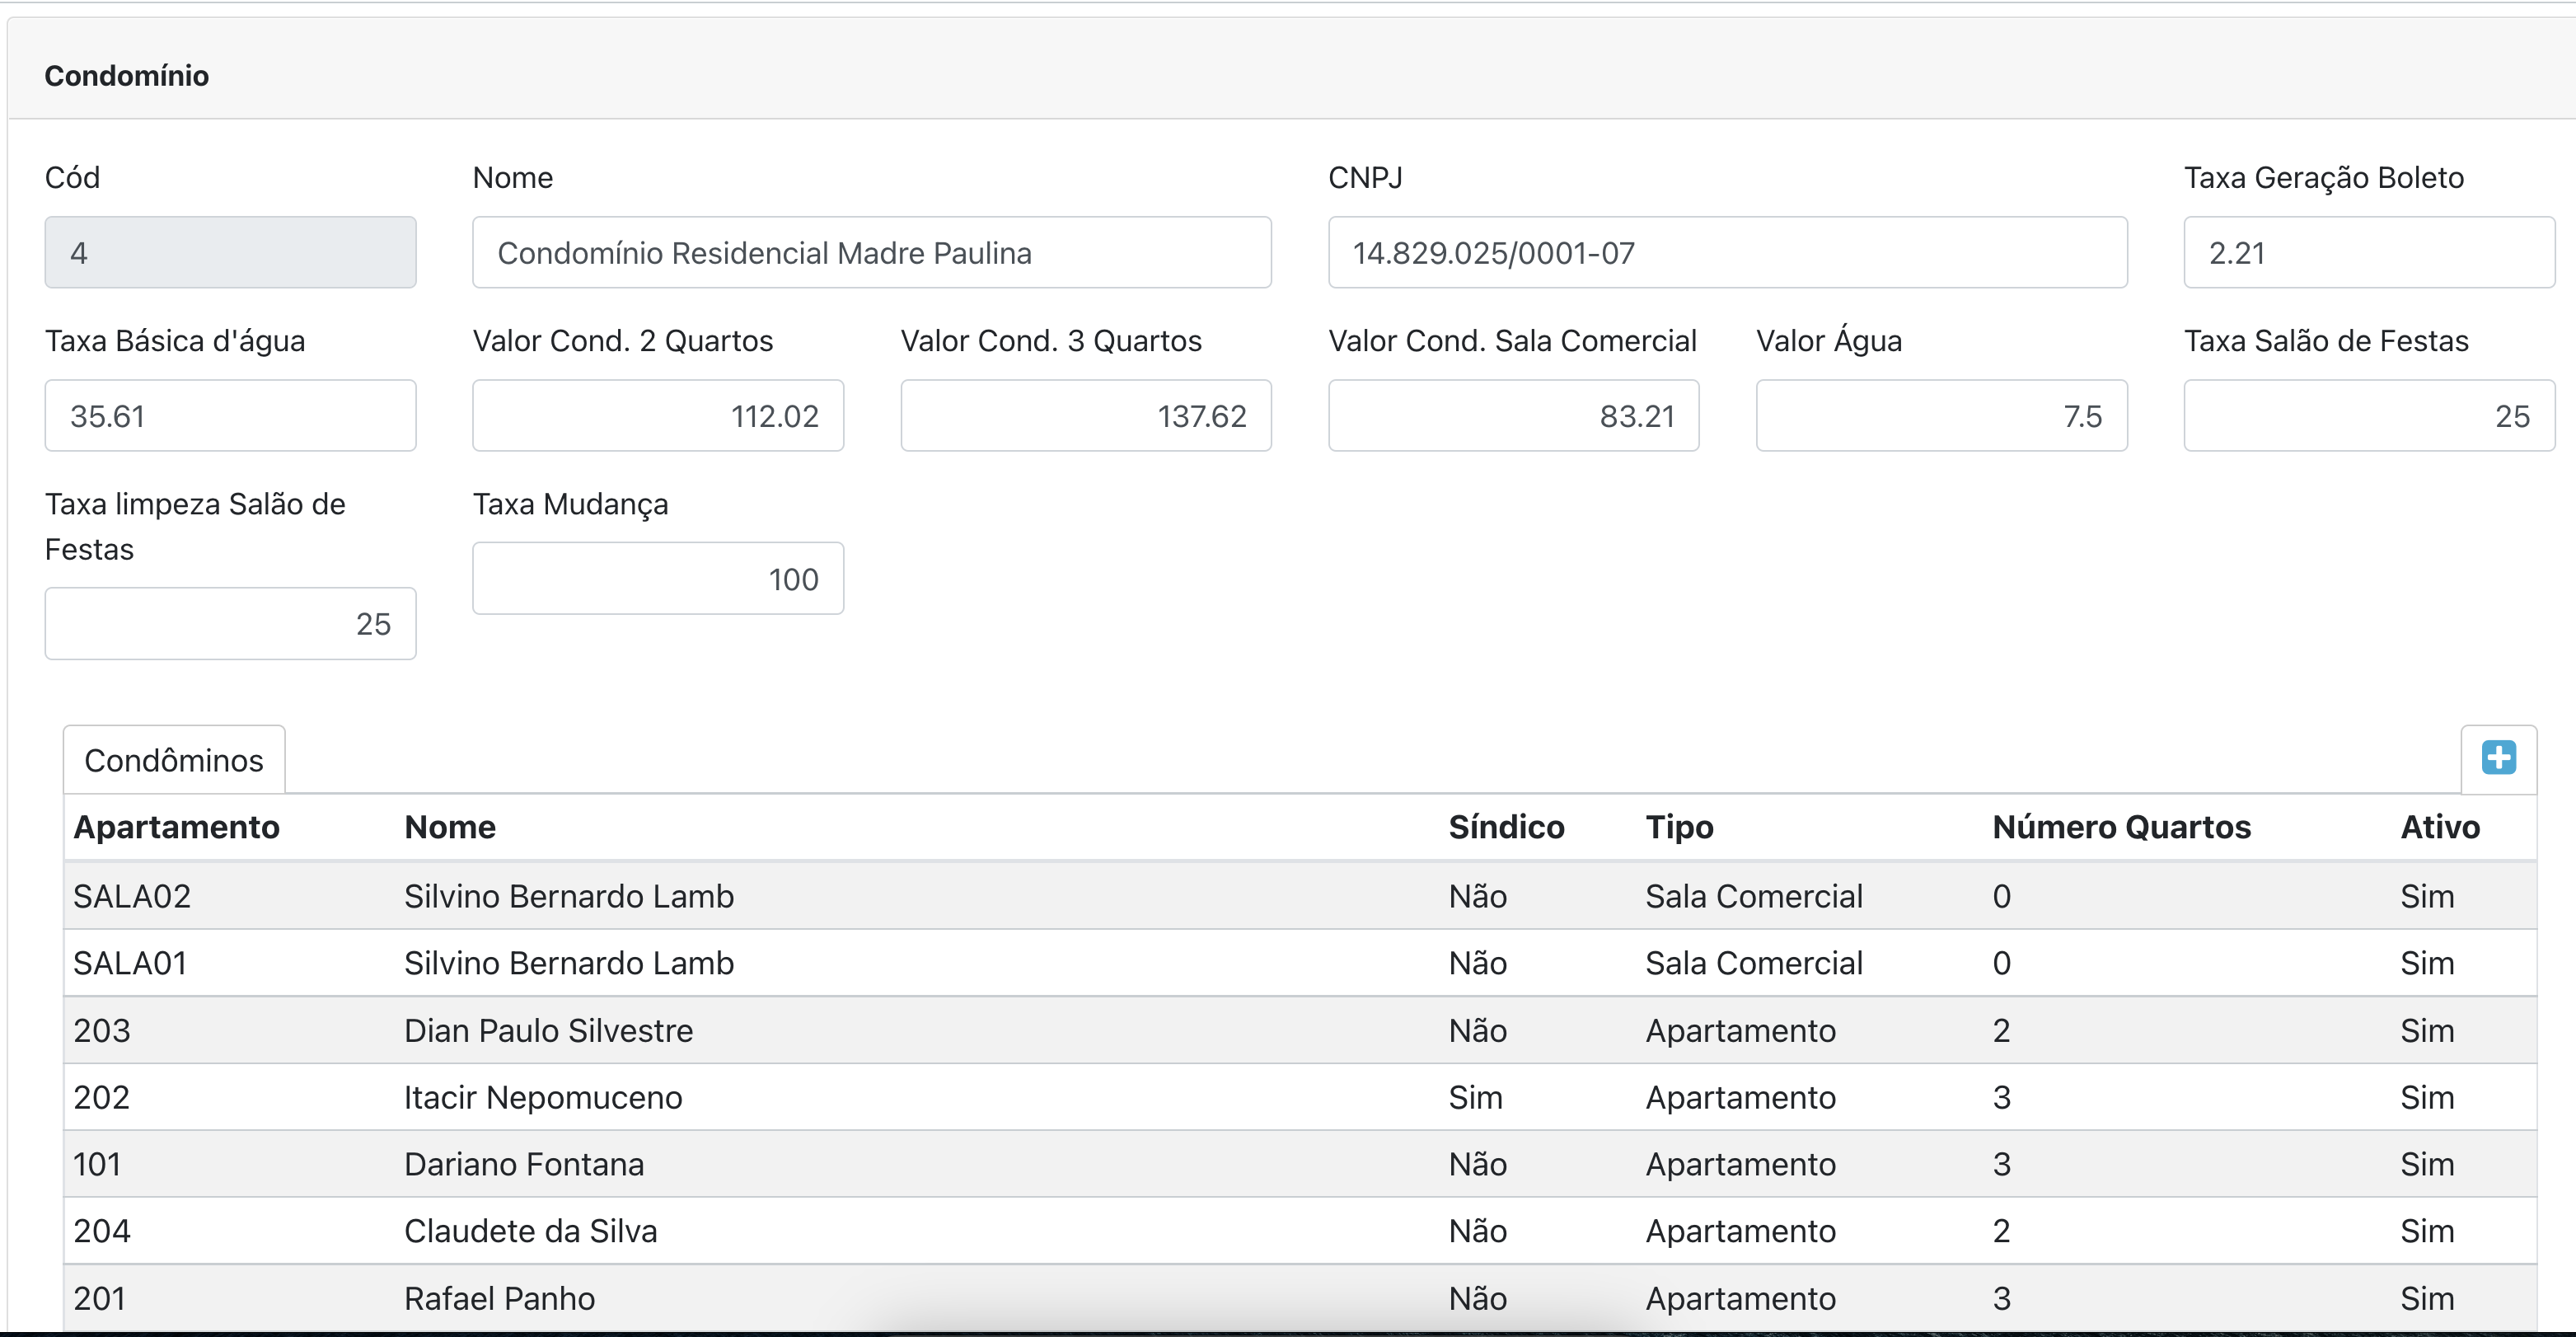
\includegraphics[width=0.9\columnwidth]{projeto/images/UI_condominio.png}
  \caption{Interface para manutenção do condomínio e condôminos}
  \label{fig:UI_condominio}
\end{figure}

\begin{figure}[!ht]
  \centering
  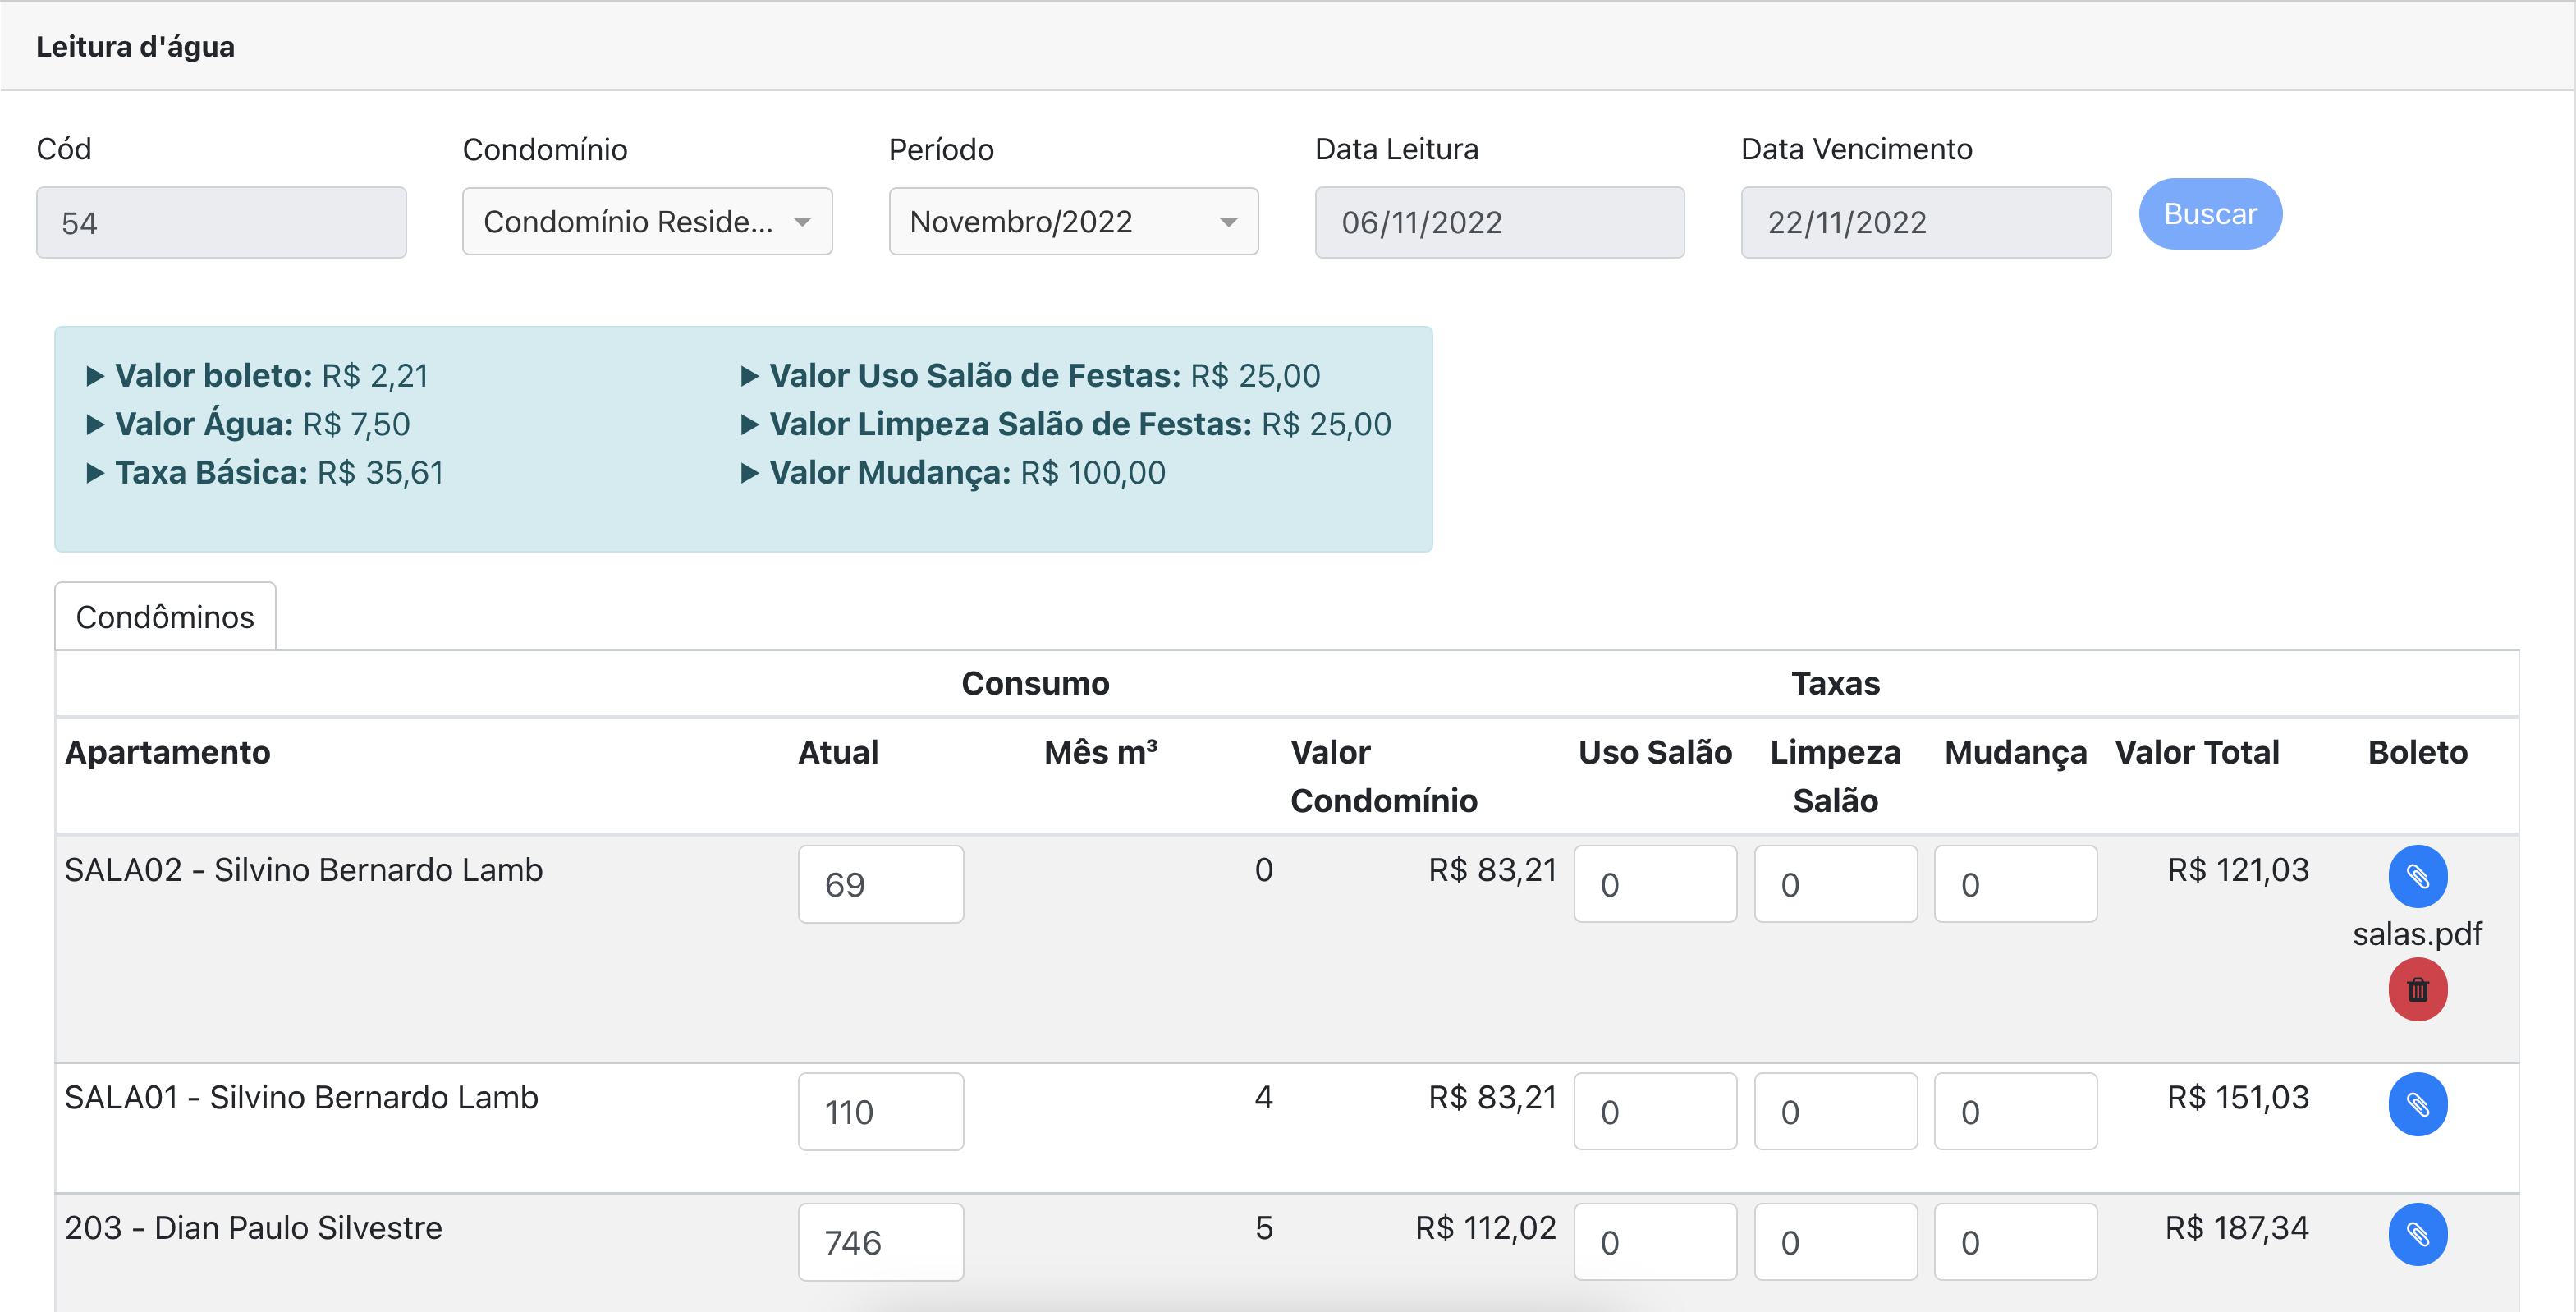
\includegraphics[width=0.9\columnwidth]{projeto/images/UI_Geracaoagua.png}
  \caption{Interface controle da leitura d`água}
  \label{fig:UI_Geracaoagua}
\end{figure}

\begin{figure}[!ht]
  \centering
  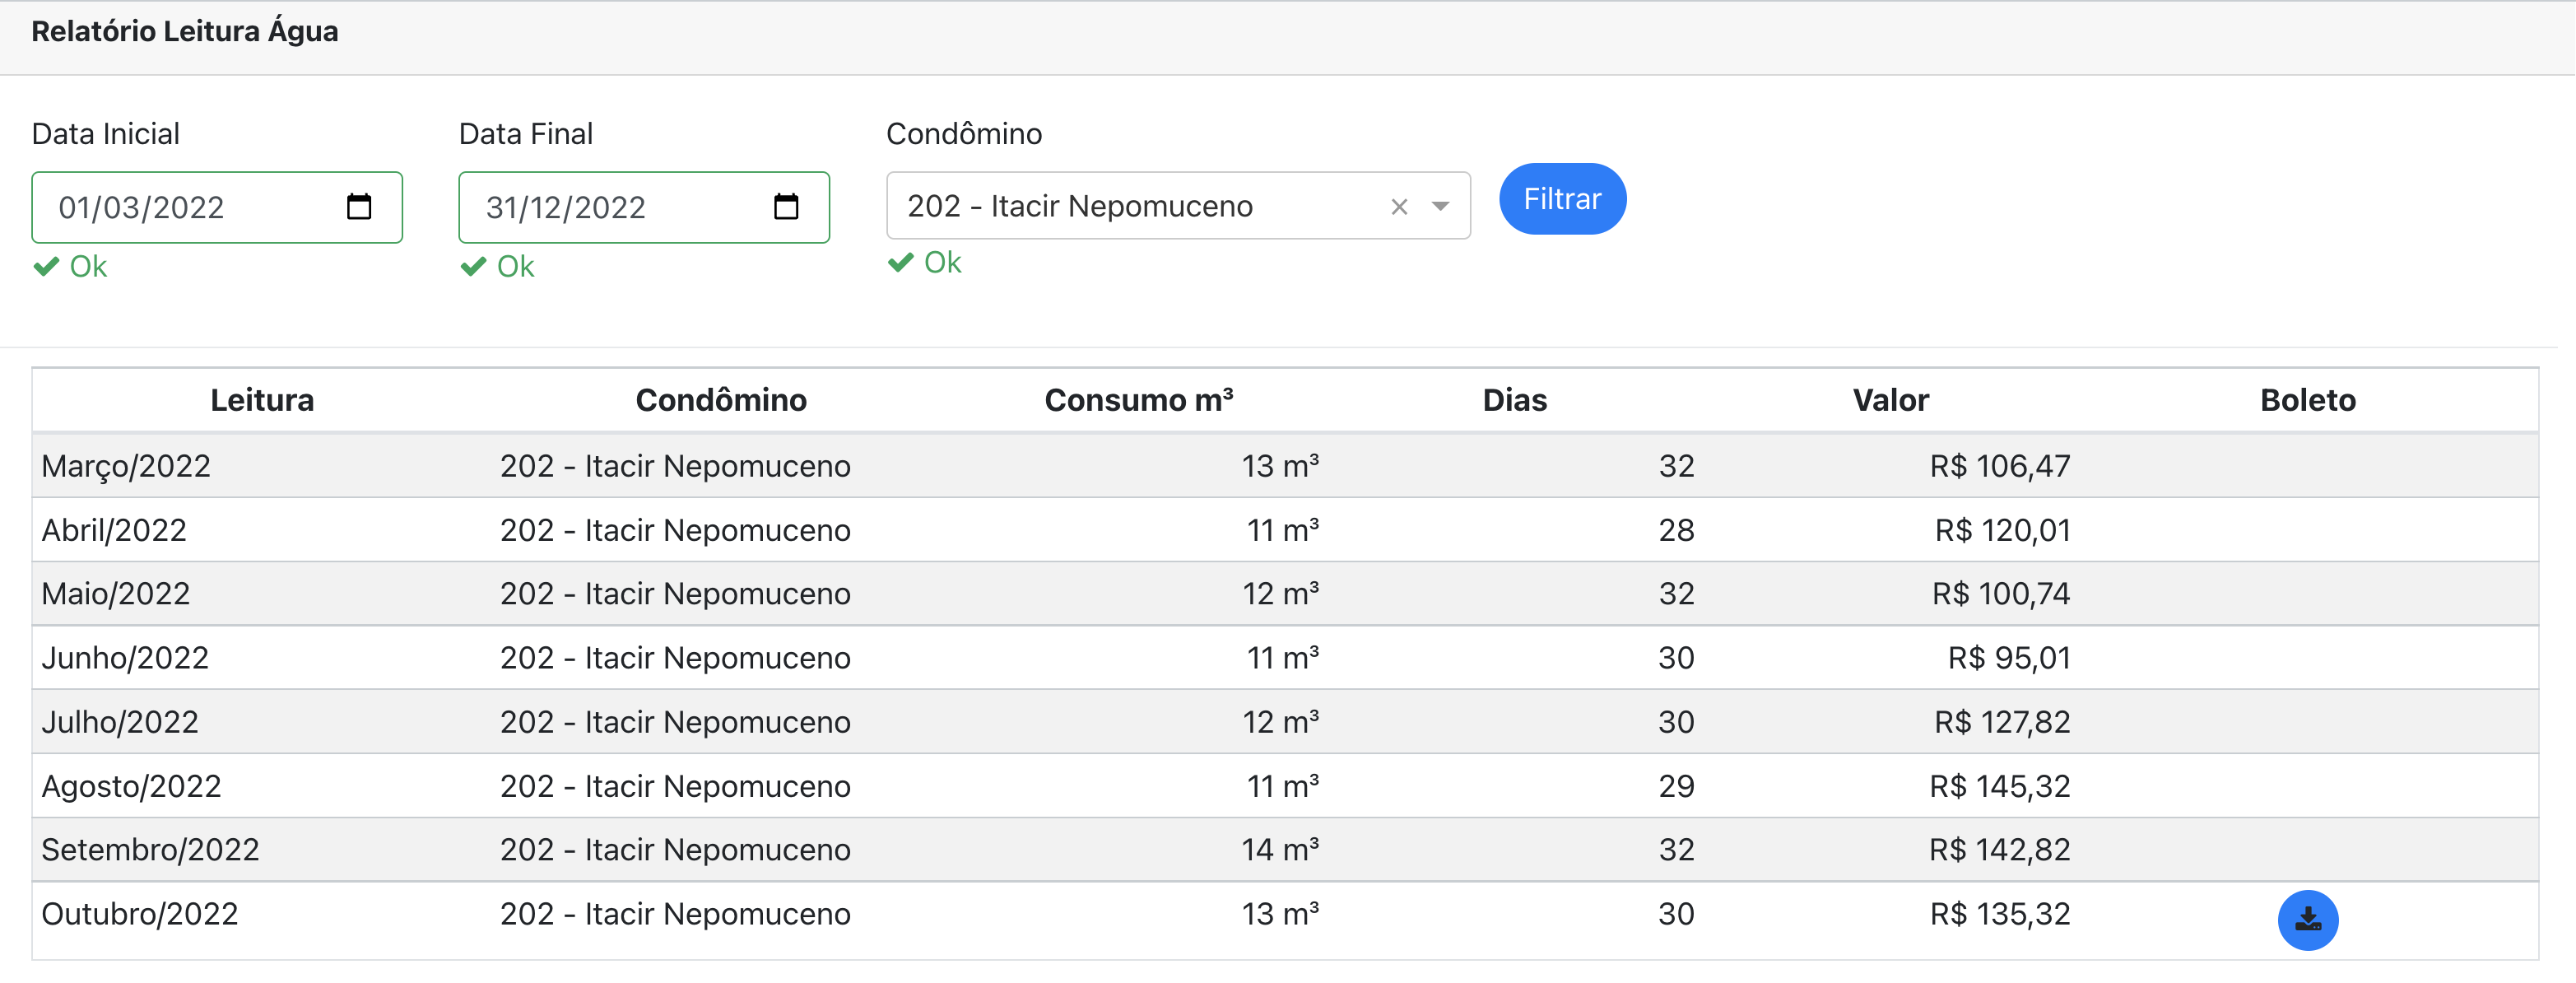
\includegraphics[width=0.9\columnwidth]{projeto/images/UI_report_consumo.png}
  \caption{Relatório leitura d`água}
  \label{fig:UI_report_consumo}
\end{figure}

\begin{figure}[!ht]
  \centering
  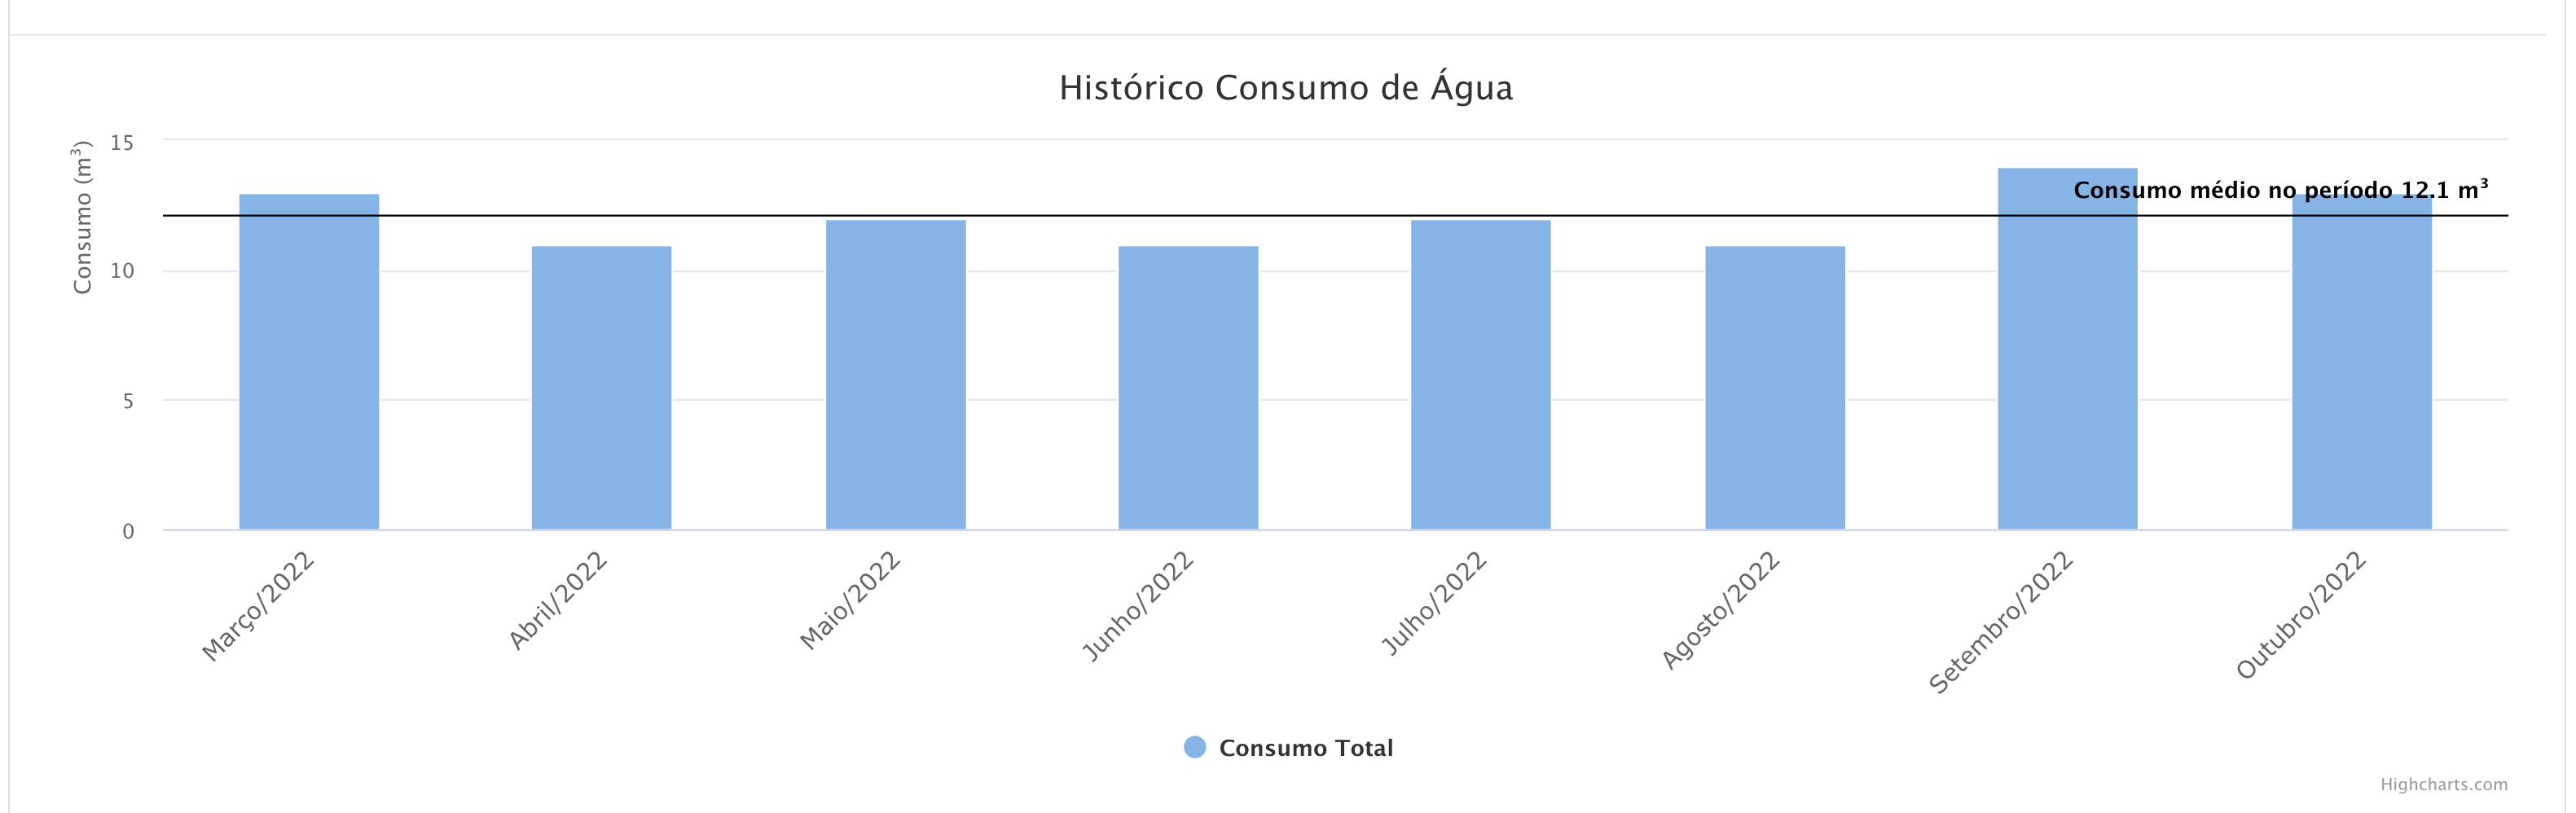
\includegraphics[width=0.9\columnwidth]{projeto/images/UI_graph_consumo.png}
  \caption{Relatório leitura d`água}
  \label{fig:UI_graph_consumo}
\end{figure}

\begin{figure}[!ht]
  \centering
  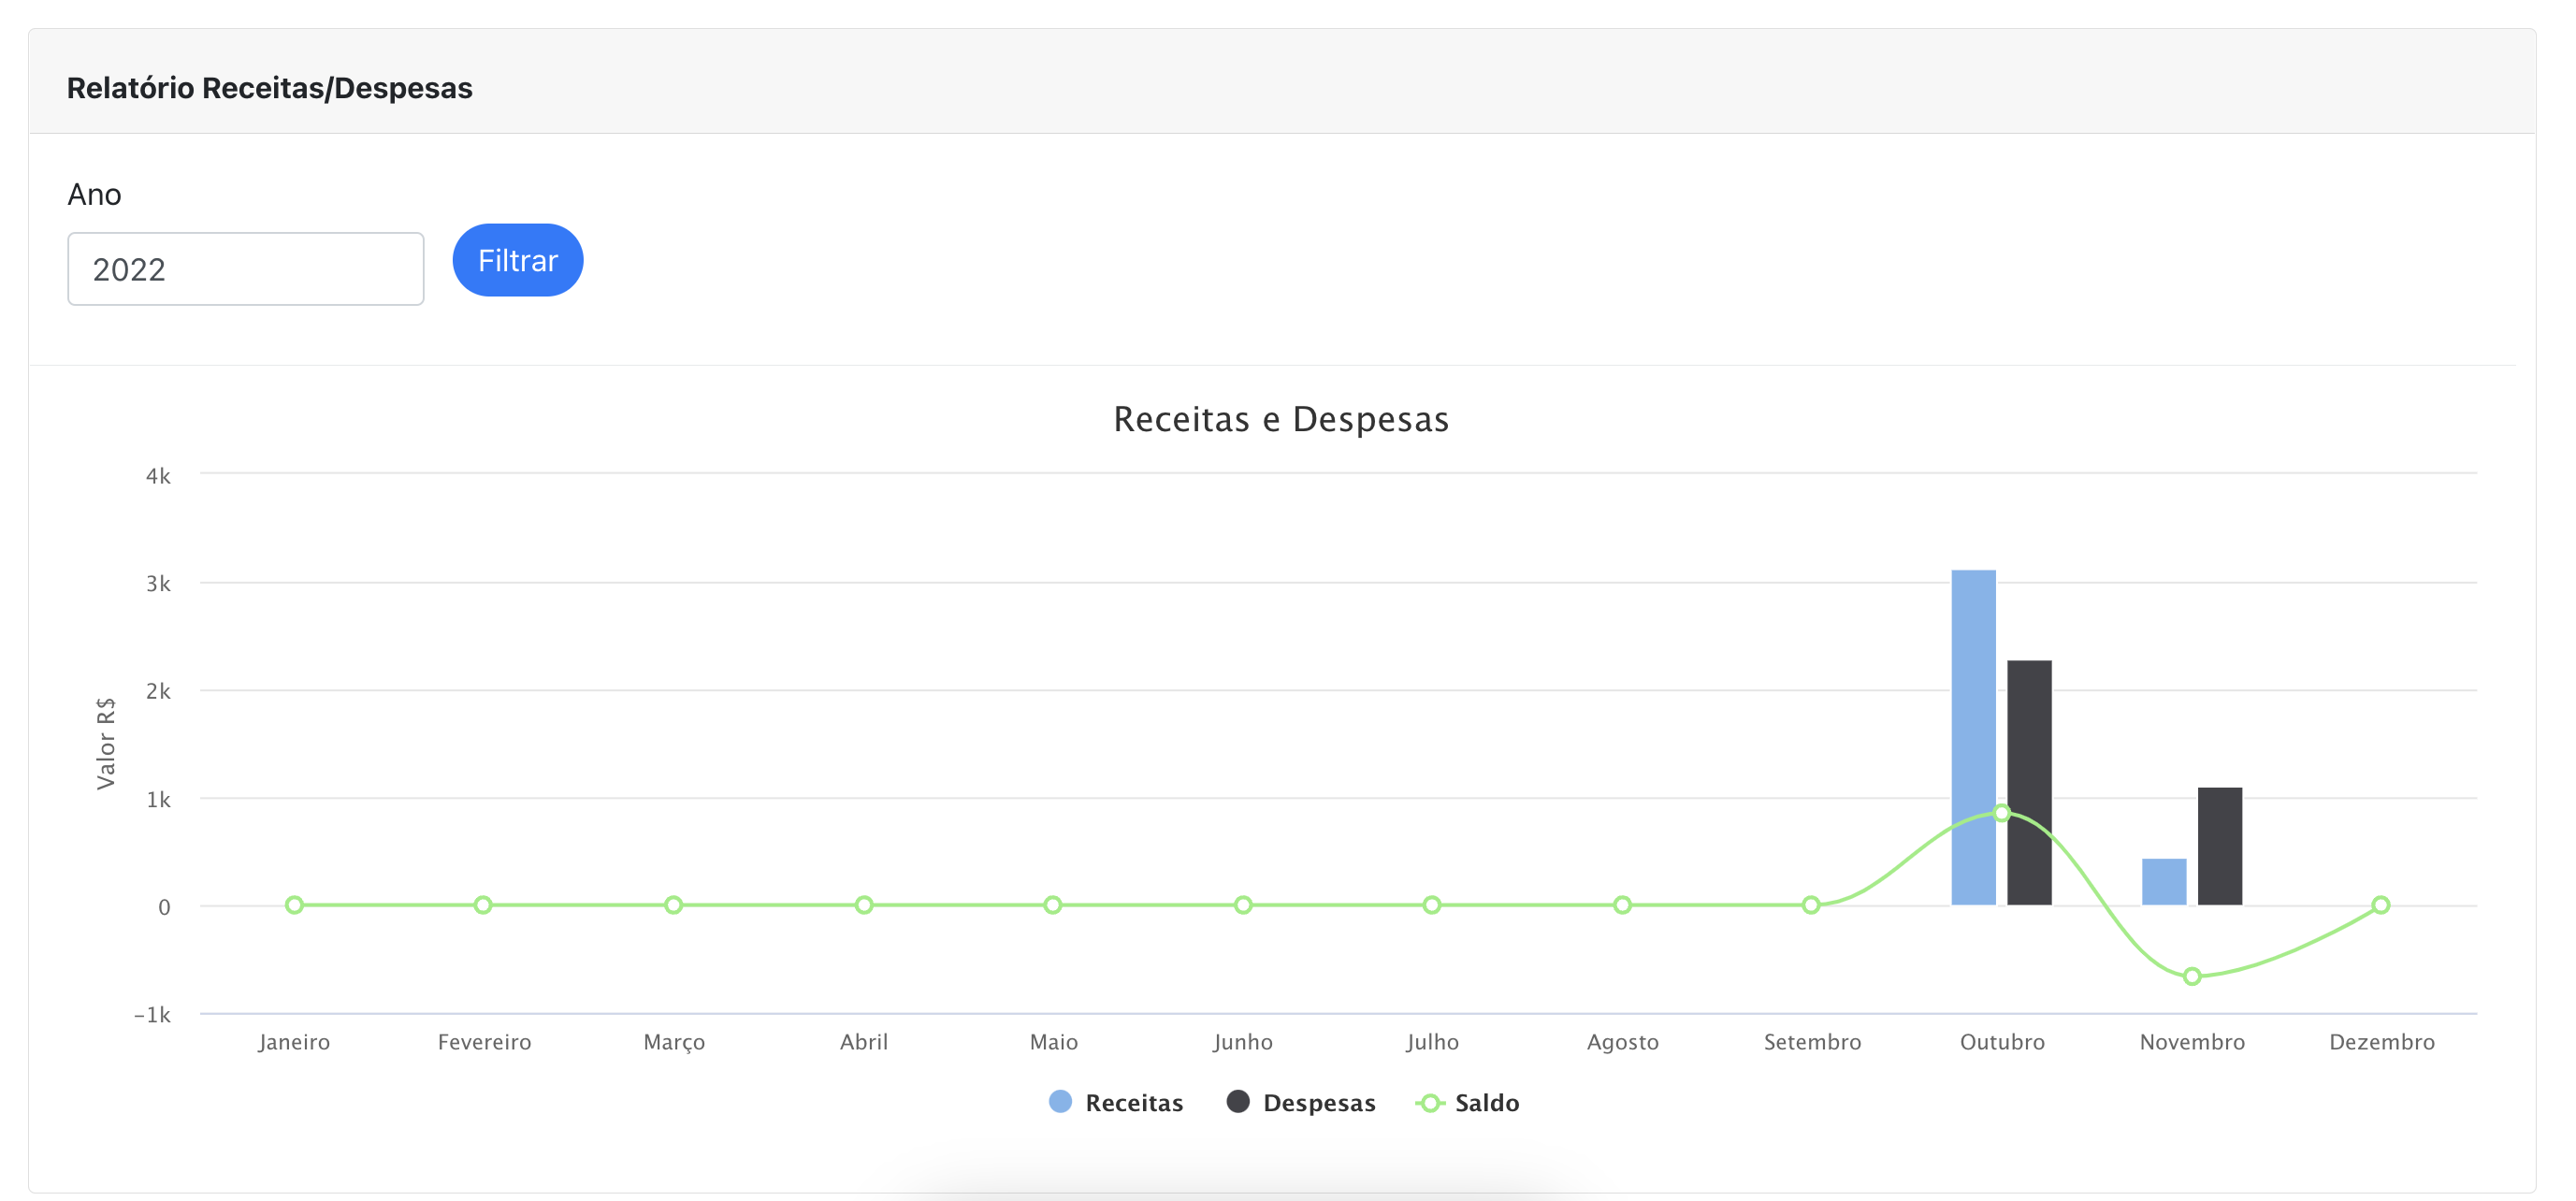
\includegraphics[width=0.9\columnwidth]{projeto/images/UI_report_cashflow.png}
  \caption{Relatório Receita/Despesas}
  \label{fig:UI_report_cashflow}
\end{figure}

\begin{table*}[!ht]
    \begin{minipage}{.4\linewidth}
        \centering
        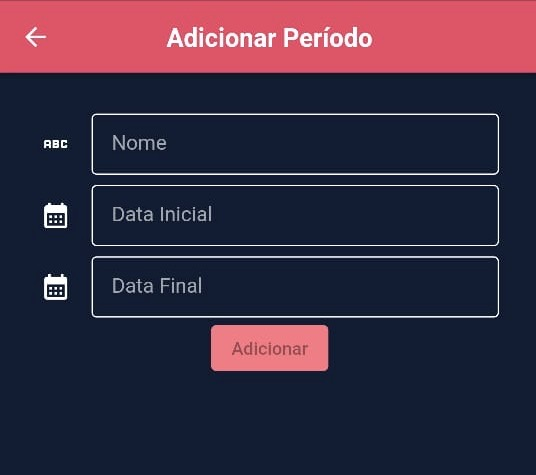
\includegraphics[width=0.9\columnwidth]{projeto/images/UI_add_period.jpeg}
        \captionof{figure}{Cadastro de períodos}
        \label{fig:UI_add_period}
    \end{minipage}
    \hfill
    \begin{minipage}{.4\linewidth}
        \centering
        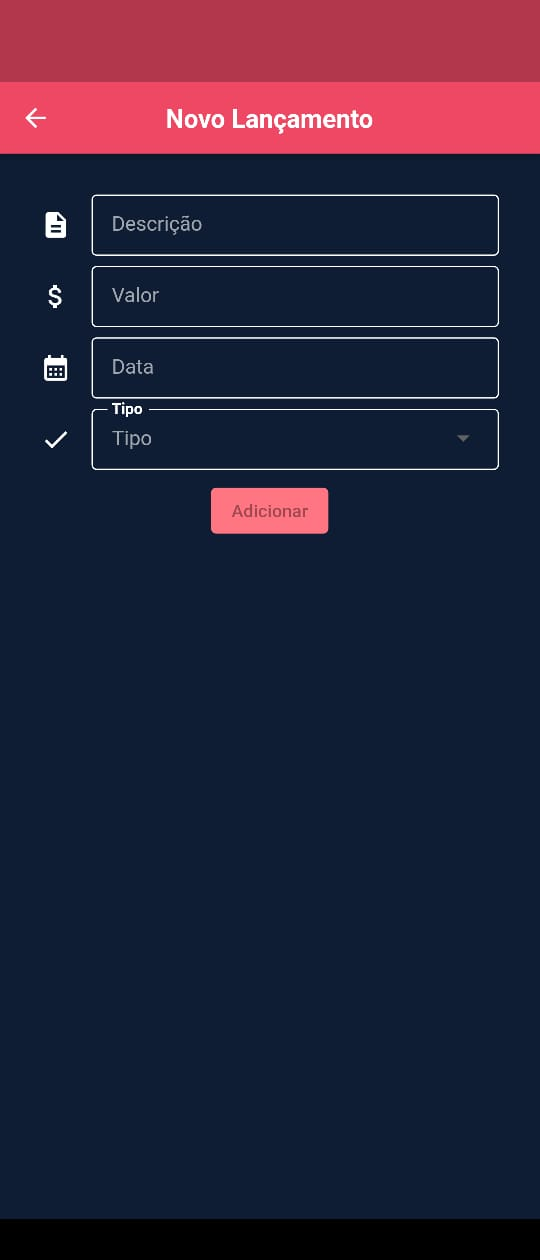
\includegraphics[width=0.9\columnwidth]{projeto/images/UI_add_period_details.jpeg}
        \captionof{figure}{Cadastro de receita/despesa}
        \label{fig:UI_add_period_details}
    \end{minipage}
\end{table*}

\begin{table*}[!ht]
    \begin{minipage}{.4\linewidth}
        \centering
        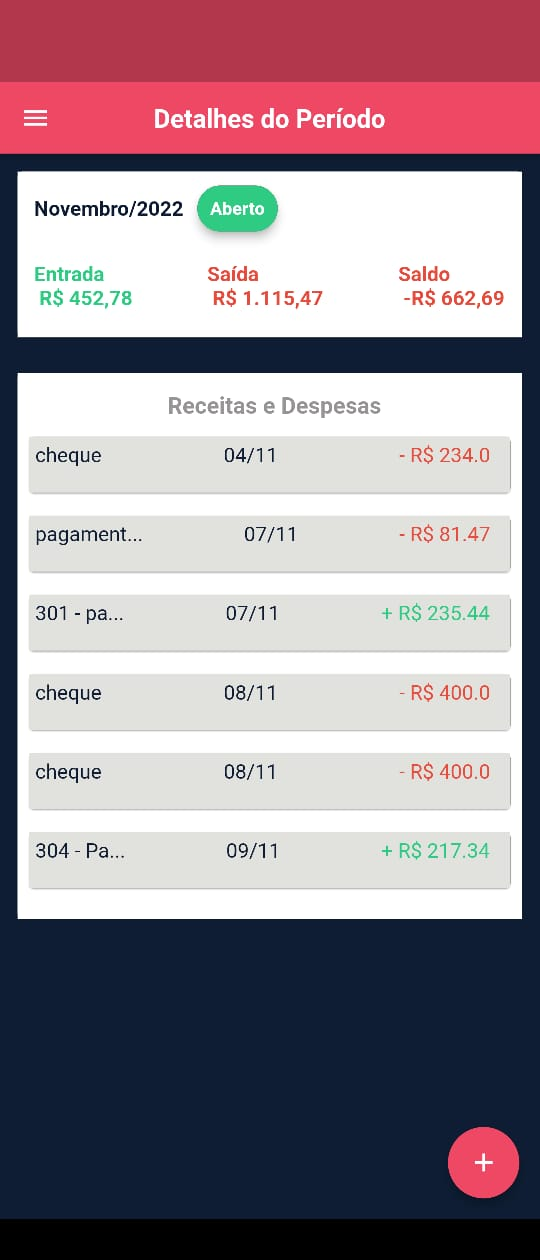
\includegraphics[width=0.9\columnwidth]{projeto/images/UI_Period_Details.jpeg}
        \captionof{figure}{Detalhes de um período}
        \label{fig:UI_Period_Details}
    \end{minipage}
\end{table*}

\end{appendices}

\end{document}
